% Map of the agent skills in Config/.cursor/skills: main skills on top,
% their reference files summarised below.
% Build: latex-scientific rule, "TikZ figures: SVG first, PDF last".
\documentclass[border=6pt]{standalone}
\usepackage{amsmath}
\usepackage{fontspec}
\usepackage{unicode-math}
\setmathfont{STIX Two Math}
\setmainfont{Noto Sans}[Ligatures=CommonOff] % match book PNGs; ligatures have no Unicode in the SVG
\usepackage{xcolor}
\usepackage{tikz}
\usetikzlibrary{positioning,fit,calc,backgrounds}
\hyphenpenalty=10000
\exhyphenpenalty=10000

\definecolor{ink}{HTML}{1C2B24}
\definecolor{green}{HTML}{0E4D3A}
\definecolor{blue}{HTML}{1D4E89}
\definecolor{orange}{HTML}{C45C26}
\definecolor{paper}{HTML}{F6F3EE}
\definecolor{grid}{HTML}{D9D3C7}

\tikzset{
  every node/.style={text=ink},
  root/.style={draw=green, fill=green, text=white, font=\bfseries,
    rounded corners=4pt, inner sep=2.5mm},
  cat/.style={draw=green, line width=0.9pt, fill=paper, font=\bfseries,
    text=green, rounded corners=4pt, minimum width=50mm, inner sep=2mm},
  skill/.style={draw=blue, line width=0.9pt, fill=white, rounded corners=3pt,
    text width=46mm, inner sep=2mm, align=left, font=\small},
  refs/.style={draw=grid, line width=0.7pt, fill=paper, rounded corners=2pt,
    text width=44mm, inner sep=1.8mm, align=left, font=\footnotesize},
  link/.style={draw=green!70, line width=0.8pt},
  sub/.style={draw=grid, line width=0.8pt},
}
% \S{name}{role}
\newcommand{\Sk}[2]{\textbf{#1}\\[0.4mm]{\footnotesize #2}}

\begin{document}
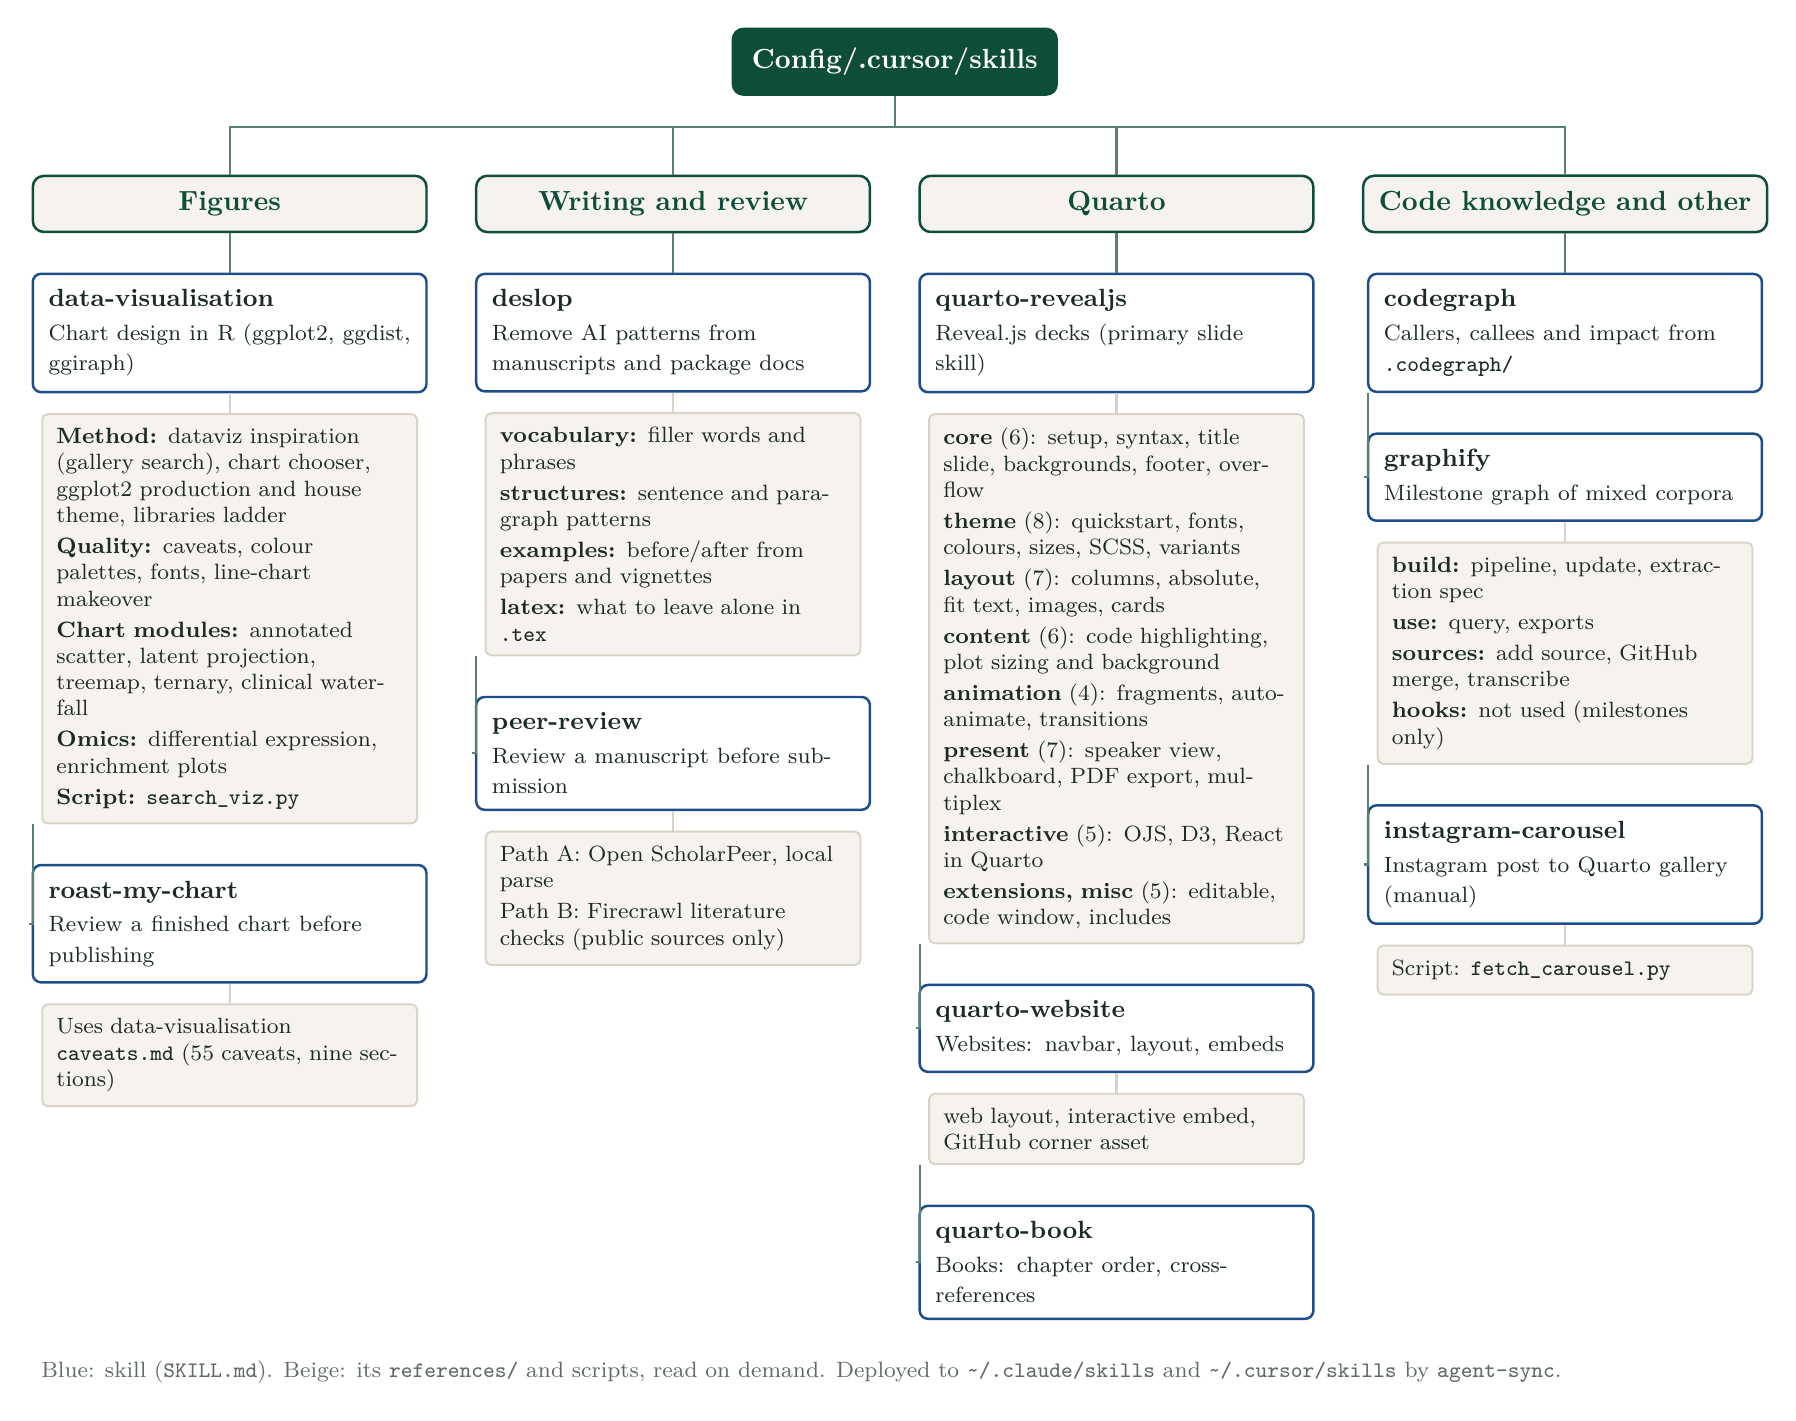
\begin{tikzpicture}[node distance=2.5mm and 6mm]

% ---- Categories -----------------------------------------------------------
\node[cat] (figs) {Figures};
\node[cat, right=of figs] (writing) {Writing and review};
\node[cat, right=of writing] (quarto) {Quarto};
\node[cat, right=of quarto] (code) {Code knowledge and other};
\node[root, anchor=south] (root) at ($(writing.north)!0.5!(quarto.north)+(0,10mm)$) {Config/.cursor/skills};
\foreach \c in {figs, writing, quarto, code}
  \draw[link] (root.south) -- ++(0,-4mm) -| (\c.north);

% ---- Figures ----------------------------------------------------------------
\node[skill, below=5mm of figs] (dv) {\Sk{data-visualisation}{Chart design in R (ggplot2, ggdist, ggiraph)}};
\node[refs, below=of dv] (dvr) {%
  \textbf{Method:} dataviz inspiration (gallery search), chart chooser, ggplot2 production and house theme, libraries ladder\\[0.6mm]
  \textbf{Quality:} caveats, colour palettes, fonts, line-chart makeover\\[0.6mm]
  \textbf{Chart modules:} annotated scatter, latent projection, treemap, ternary, clinical waterfall\\[0.6mm]
  \textbf{Omics:} differential expression, enrichment plots\\[0.6mm]
  \textbf{Script:} \texttt{search\_viz.py}};
\node[skill, below=5mm of dvr] (roast) {\Sk{roast-my-chart}{Review a finished chart before publishing}};
\node[refs, below=of roast] (roastr) {Uses data-visualisation \texttt{caveats.md} (55 caveats, nine sections)};

% ---- Writing and review -----------------------------------------------------
\node[skill, below=5mm of writing] (deslop) {\Sk{deslop}{Remove AI patterns from manuscripts and package docs}};
\node[refs, below=of deslop] (deslopr) {%
  \textbf{vocabulary:} filler words and phrases\\[0.6mm]
  \textbf{structures:} sentence and paragraph patterns\\[0.6mm]
  \textbf{examples:} before/after from papers and vignettes\\[0.6mm]
  \textbf{latex:} what to leave alone in \texttt{.tex}};
\node[skill, below=5mm of deslopr] (review) {\Sk{peer-review}{Review a manuscript before submission}};
\node[refs, below=of review] (reviewr) {Path A: Open ScholarPeer, local parse\\[0.6mm]
  Path B: Firecrawl literature checks (public sources only)};

% ---- Quarto -------------------------------------------------------------------
\node[skill, below=5mm of quarto] (reveal) {\Sk{quarto-revealjs}{Reveal.js decks (primary slide skill)}};
\node[refs, below=of reveal] (revealr) {%
  \textbf{core} (6): setup, syntax, title slide, backgrounds, footer, overflow\\[0.6mm]
  \textbf{theme} (8): quickstart, fonts, colours, sizes, SCSS, variants\\[0.6mm]
  \textbf{layout} (7): columns, absolute, fit text, images, cards\\[0.6mm]
  \textbf{content} (6): code highlighting, plot sizing and background\\[0.6mm]
  \textbf{animation} (4): fragments, auto-animate, transitions\\[0.6mm]
  \textbf{present} (7): speaker view, chalkboard, PDF export, multiplex\\[0.6mm]
  \textbf{interactive} (5): OJS, D3, React in Quarto\\[0.6mm]
  \textbf{extensions, misc} (5): editable, code window, includes};
\node[skill, below=5mm of revealr] (web) {\Sk{quarto-website}{Websites: navbar, layout, embeds}};
\node[refs, below=of web] (webr) {web layout, interactive embed, GitHub corner asset};
\node[skill, below=5mm of webr] (book) {\Sk{quarto-book}{Books: chapter order, cross-references}};

% ---- Code knowledge and other --------------------------------------------------
\node[skill, below=5mm of code] (cg) {\Sk{codegraph}{Callers, callees and impact from \texttt{.codegraph/}}};
\node[skill, below=5mm of cg] (gf) {\Sk{graphify}{Milestone graph of mixed corpora}};
\node[refs, below=of gf] (gfr) {%
  \textbf{build:} pipeline, update, extraction spec\\[0.6mm]
  \textbf{use:} query, exports\\[0.6mm]
  \textbf{sources:} add source, GitHub merge, transcribe\\[0.6mm]
  \textbf{hooks:} not used (milestones only)};
\node[skill, below=5mm of gfr] (insta) {\Sk{instagram-carousel}{Instagram post to Quarto gallery (manual)}};
\node[refs, below=of insta] (instar) {Script: \texttt{fetch\_carousel.py}};

% ---- Links ----------------------------------------------------------------------
\foreach \c/\s in {figs/dv, writing/deslop, quarto/reveal, code/cg}
  \draw[link] (\c.south) -- (\s.north);
\foreach \a/\b in {dv/dvr, roast/roastr, deslop/deslopr, review/reviewr,
                   reveal/revealr, web/webr, gf/gfr, insta/instar}
  \draw[sub] (\a.south) -- (\b.north);
\foreach \a/\b in {dvr/roast, deslopr/review, revealr/web, webr/book,
                   cg/gf, gfr/insta}
  \draw[link] ([xshift=-25mm]\a.south) |- ([xshift=-1pt]\b.west);

\node[font=\footnotesize, text=ink!70, anchor=north west, align=left]
  at ($(figs.west |- book.south)+(0,-4mm)$)
  {Blue: skill (\texttt{SKILL.md}). Beige: its \texttt{references/} and scripts, read on demand.
   Deployed to \texttt{\textasciitilde/.claude/skills} and \texttt{\textasciitilde/.cursor/skills} by \texttt{agent-sync}.};
\end{tikzpicture}
\end{document}
